%%%%%%%%%%%%%%%%%%%%%%%%%%%%%%%%%%%%%%%%%%%%%%%%%%%%%%%%%%%%%%%%%%%%%%%%%%%%%%%%%%%%%%%%%%%%%%%%%%%%%%%%%%%%%%%%%%%%%%%%%%%%%%%%%%%%%%%%%%%%%%%%%%%%%%%%%%%%%%%%%%%
% Written By Michael Brodskiy
% Class: Fundamentals of Linear Systems
% Professor: I. Salama
%%%%%%%%%%%%%%%%%%%%%%%%%%%%%%%%%%%%%%%%%%%%%%%%%%%%%%%%%%%%%%%%%%%%%%%%%%%%%%%%%%%%%%%%%%%%%%%%%%%%%%%%%%%%%%%%%%%%%%%%%%%%%%%%%%%%%%%%%%%%%%%%%%%%%%%%%%%%%%%%%%%

\include{Includes.tex}

\title{Homework 2}
\date{\today}
\author{Michael Brodskiy\\ \small Professor: I. Salama}

\begin{document}

\maketitle

\begin{enumerate}

  \item

    \begin{enumerate}[label=\textbf{\Roman*.}]

      \item 

        \begin{enumerate}[label=\alph*)]

          \item 

            We begin by sketching $x[n-2]$, which generates a rightward shift of $2$:

            \begin{figure}[H]
              \centering
              \include{Figures/H2P1a1.tex}
              \caption{$x[n-2]$}
              \label{fig:1}
            \end{figure}

            We then apply the delta function to filter out only the value at $n=2$:

            \begin{figure}[H]
              \centering
              \include{Figures/H2P1a2.tex}
              \caption{$x[n-2]\delta(n-2)$}
              \label{fig:2}
            \end{figure}

          \item 

            Once again, the delta extracts the value at $n=2$, except the function is no longer shifted. This gives us the following graph:

            \begin{figure}[H]
              \centering
              \tikzset{every picture/.style={line width=0.75pt}} %set default line width to 0.75pt        

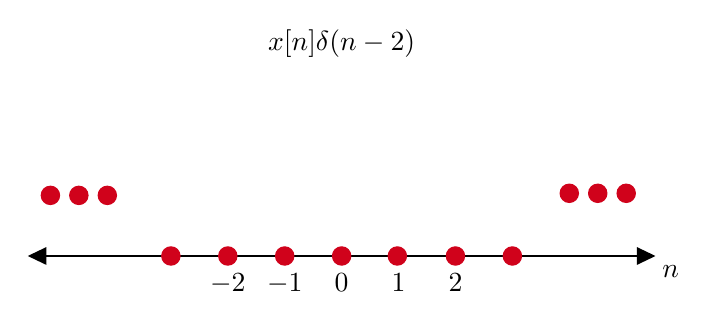
\begin{tikzpicture}[x=0.75pt,y=0.75pt,yscale=-1,xscale=1]
%uncomment if require: \path (0,437); %set diagram left start at 0, and has height of 437

%Straight Lines [id:da6728625031917905] 
\draw    (437.71,170) -- (141.29,170) ;
\draw [shift={(138.29,170)}, rotate = 360] [fill={rgb, 255:red, 0; green, 0; blue, 0 }  ][line width=0.08]  [draw opacity=0] (8.93,-4.29) -- (0,0) -- (8.93,4.29) -- cycle    ;
\draw [shift={(440.71,170)}, rotate = 180] [fill={rgb, 255:red, 0; green, 0; blue, 0 }  ][line width=0.08]  [draw opacity=0] (8.93,-4.29) -- (0,0) -- (8.93,4.29) -- cycle    ;
%Shape: Circle [id:dp16680741947391897] 
\draw  [color={rgb, 255:red, 208; green, 2; blue, 27 }  ,draw opacity=1 ][fill={rgb, 255:red, 208; green, 2; blue, 27 }  ,fill opacity=1 ] (202.81,170) .. controls (202.81,167.56) and (204.79,165.58) .. (207.24,165.58) .. controls (209.68,165.58) and (211.66,167.56) .. (211.66,170) .. controls (211.66,172.44) and (209.68,174.42) .. (207.24,174.42) .. controls (204.79,174.42) and (202.81,172.44) .. (202.81,170) -- cycle ;
%Shape: Circle [id:dp24325412264442625] 
\draw  [color={rgb, 255:red, 208; green, 2; blue, 27 }  ,draw opacity=1 ][fill={rgb, 255:red, 208; green, 2; blue, 27 }  ,fill opacity=1 ] (367.34,170) .. controls (367.34,167.56) and (369.32,165.58) .. (371.76,165.58) .. controls (374.21,165.58) and (376.19,167.56) .. (376.19,170) .. controls (376.19,172.44) and (374.21,174.42) .. (371.76,174.42) .. controls (369.32,174.42) and (367.34,172.44) .. (367.34,170) -- cycle ;
%Shape: Circle [id:dp3570850369681069] 
\draw  [color={rgb, 255:red, 208; green, 2; blue, 27 }  ,draw opacity=1 ][fill={rgb, 255:red, 208; green, 2; blue, 27 }  ,fill opacity=1 ] (394.76,139.79) .. controls (394.76,137.35) and (396.74,135.37) .. (399.19,135.37) .. controls (401.63,135.37) and (403.61,137.35) .. (403.61,139.79) .. controls (403.61,142.23) and (401.63,144.21) .. (399.19,144.21) .. controls (396.74,144.21) and (394.76,142.23) .. (394.76,139.79) -- cycle ;
%Shape: Circle [id:dp3297830684019689] 
\draw  [color={rgb, 255:red, 208; green, 2; blue, 27 }  ,draw opacity=1 ][fill={rgb, 255:red, 208; green, 2; blue, 27 }  ,fill opacity=1 ] (408.47,139.79) .. controls (408.47,137.35) and (410.45,135.37) .. (412.9,135.37) .. controls (415.34,135.37) and (417.32,137.35) .. (417.32,139.79) .. controls (417.32,142.23) and (415.34,144.21) .. (412.9,144.21) .. controls (410.45,144.21) and (408.47,142.23) .. (408.47,139.79) -- cycle ;
%Shape: Circle [id:dp12503088297139797] 
\draw  [color={rgb, 255:red, 208; green, 2; blue, 27 }  ,draw opacity=1 ][fill={rgb, 255:red, 208; green, 2; blue, 27 }  ,fill opacity=1 ] (422.19,139.79) .. controls (422.19,137.35) and (424.16,135.37) .. (426.61,135.37) .. controls (429.05,135.37) and (431.03,137.35) .. (431.03,139.79) .. controls (431.03,142.23) and (429.05,144.21) .. (426.61,144.21) .. controls (424.16,144.21) and (422.19,142.23) .. (422.19,139.79) -- cycle ;
%Shape: Circle [id:dp7532419367276733] 
\draw  [color={rgb, 255:red, 208; green, 2; blue, 27 }  ,draw opacity=1 ][fill={rgb, 255:red, 208; green, 2; blue, 27 }  ,fill opacity=1 ] (144.76,140.79) .. controls (144.76,138.35) and (146.74,136.37) .. (149.19,136.37) .. controls (151.63,136.37) and (153.61,138.35) .. (153.61,140.79) .. controls (153.61,143.23) and (151.63,145.21) .. (149.19,145.21) .. controls (146.74,145.21) and (144.76,143.23) .. (144.76,140.79) -- cycle ;
%Shape: Circle [id:dp8234155158894582] 
\draw  [color={rgb, 255:red, 208; green, 2; blue, 27 }  ,draw opacity=1 ][fill={rgb, 255:red, 208; green, 2; blue, 27 }  ,fill opacity=1 ] (158.47,140.79) .. controls (158.47,138.35) and (160.45,136.37) .. (162.9,136.37) .. controls (165.34,136.37) and (167.32,138.35) .. (167.32,140.79) .. controls (167.32,143.23) and (165.34,145.21) .. (162.9,145.21) .. controls (160.45,145.21) and (158.47,143.23) .. (158.47,140.79) -- cycle ;
%Shape: Circle [id:dp3922736373189596] 
\draw  [color={rgb, 255:red, 208; green, 2; blue, 27 }  ,draw opacity=1 ][fill={rgb, 255:red, 208; green, 2; blue, 27 }  ,fill opacity=1 ] (172.19,140.79) .. controls (172.19,138.35) and (174.16,136.37) .. (176.61,136.37) .. controls (179.05,136.37) and (181.03,138.35) .. (181.03,140.79) .. controls (181.03,143.23) and (179.05,145.21) .. (176.61,145.21) .. controls (174.16,145.21) and (172.19,143.23) .. (172.19,140.79) -- cycle ;
%Shape: Circle [id:dp08799827139095029] 
\draw  [color={rgb, 255:red, 208; green, 2; blue, 27 }  ,draw opacity=1 ][fill={rgb, 255:red, 208; green, 2; blue, 27 }  ,fill opacity=1 ] (311.92,170) .. controls (311.92,167.56) and (313.9,165.58) .. (316.34,165.58) .. controls (318.78,165.58) and (320.76,167.56) .. (320.76,170) .. controls (320.76,172.44) and (318.78,174.42) .. (316.34,174.42) .. controls (313.9,174.42) and (311.92,172.44) .. (311.92,170) -- cycle ;
%Shape: Circle [id:dp17224497070467182] 
\draw  [color={rgb, 255:red, 208; green, 2; blue, 27 }  ,draw opacity=1 ][fill={rgb, 255:red, 208; green, 2; blue, 27 }  ,fill opacity=1 ] (285.08,170) .. controls (285.08,167.56) and (287.06,165.58) .. (289.5,165.58) .. controls (291.94,165.58) and (293.92,167.56) .. (293.92,170) .. controls (293.92,172.44) and (291.94,174.42) .. (289.5,174.42) .. controls (287.06,174.42) and (285.08,172.44) .. (285.08,170) -- cycle ;
%Shape: Circle [id:dp6391167979037089] 
\draw  [color={rgb, 255:red, 208; green, 2; blue, 27 }  ,draw opacity=1 ][fill={rgb, 255:red, 208; green, 2; blue, 27 }  ,fill opacity=1 ] (339.92,170) .. controls (339.92,167.56) and (341.9,165.58) .. (344.34,165.58) .. controls (346.78,165.58) and (348.76,167.56) .. (348.76,170) .. controls (348.76,172.44) and (346.78,174.42) .. (344.34,174.42) .. controls (341.9,174.42) and (339.92,172.44) .. (339.92,170) -- cycle ;
%Shape: Circle [id:dp17888419586842064] 
\draw  [color={rgb, 255:red, 208; green, 2; blue, 27 }  ,draw opacity=1 ][fill={rgb, 255:red, 208; green, 2; blue, 27 }  ,fill opacity=1 ] (257.66,170) .. controls (257.66,167.56) and (259.64,165.58) .. (262.08,165.58) .. controls (264.52,165.58) and (266.5,167.56) .. (266.5,170) .. controls (266.5,172.44) and (264.52,174.42) .. (262.08,174.42) .. controls (259.64,174.42) and (257.66,172.44) .. (257.66,170) -- cycle ;
%Shape: Circle [id:dp5735202823595982] 
\draw  [color={rgb, 255:red, 208; green, 2; blue, 27 }  ,draw opacity=1 ][fill={rgb, 255:red, 208; green, 2; blue, 27 }  ,fill opacity=1 ] (230.24,170) .. controls (230.24,167.56) and (232.22,165.58) .. (234.66,165.58) .. controls (237.1,165.58) and (239.08,167.56) .. (239.08,170) .. controls (239.08,172.44) and (237.1,174.42) .. (234.66,174.42) .. controls (232.22,174.42) and (230.24,172.44) .. (230.24,170) -- cycle ;

% Text Node
\draw (442.71,173.4) node [anchor=north west][inner sep=0.75pt]    {$n$};
% Text Node
\draw (289.5,75.6) node [anchor=south] [inner sep=0.75pt]    {$x[ n] \delta ( n-2)$};
% Text Node
\draw (234.66,177.4) node [anchor=north] [inner sep=0.75pt]    {$-2$};
% Text Node
\draw (262.08,177.4) node [anchor=north] [inner sep=0.75pt]    {$-1$};
% Text Node
\draw (289.5,177.4) node [anchor=north] [inner sep=0.75pt]    {$0$};
% Text Node
\draw (316.92,177.4) node [anchor=north] [inner sep=0.75pt]    {$1$};
% Text Node
\draw (344.34,177.4) node [anchor=north] [inner sep=0.75pt]    {$2$};


\end{tikzpicture}

              \caption{$x[n]\delta(n-2)$}
              \label{fig:3}
            \end{figure}

          \item 

            We begin by referencing Figure \ref{fig:1}. The step function then draws all values left (due to the negative sign) of and including $n=1$. This gives us:

            \begin{figure}[H]
              \centering
              \include{Figures/H2P1c.tex}
              \caption{$x[n-2]u(1-n)$}
              \label{fig:4}
            \end{figure}

        \end{enumerate}

      \item 

        Although, due to the step function, we can adjust the bounds to:

        $$\int_{-2}^{\infty}5t^2\cos(\pi t)\delta(t-2)\,dt$$

        This is unnecessary, as the sifting property makes this a function evaluated at $t=2$:

        $$\int_{-\infty}^{\infty}5t^2\cos(\pi t)u(t+2)\delta(t-2)\,dt=5t^2\cos(\pi t)\Big|_{t=2}$$

        This gives us:

        $$5(2)^2\cos(2\pi)=20$$

        Thus, we find:

        $$\boxed{\int_{-\infty}^{\infty}5t^2\cos(\pi t)u(t+2)\delta(t-2)\,dt=20}$$

    \end{enumerate}

  \item

    For this problem, we begin by changing the summation to a unit step function. The summation given is:

    $$\sum_{k=2}^{\infty}\delta[n-4-k]$$

    We know that, to equal one, the delta function needs to be evaluated at a point where:

    $$n-4-k\geq 0$$
    $$n\geq k+4$$

    The smallest such value occurs when:

    $$n=6$$

    Thus, we can say that the function $x[n]=1$ from $-\infty$ to $5$, and zero otherwise. This can be written as:

    $$x[n]=u(5-n)$$

    Which means:

    $$\boxed{M=-1;\quad n_o=-5}$$

  \item

    The function $y(t)$ may be rewritten as:

    $$y(t)=\left\{\begin{matrix} 0, & t<-1\\ 2, & -1\leq t< 4\\ 0, & t\geq 4\end{matrix}$$

      \begin{center}
        or
      \end{center}

      \vspace{-15pt}

      $$y(t)=2u(t+1)-2u(t-4)$$

      This would look like:

      \begin{figure}[H]
        \centering
        \tikzset{every picture/.style={line width=0.75pt}} %set default line width to 0.75pt        

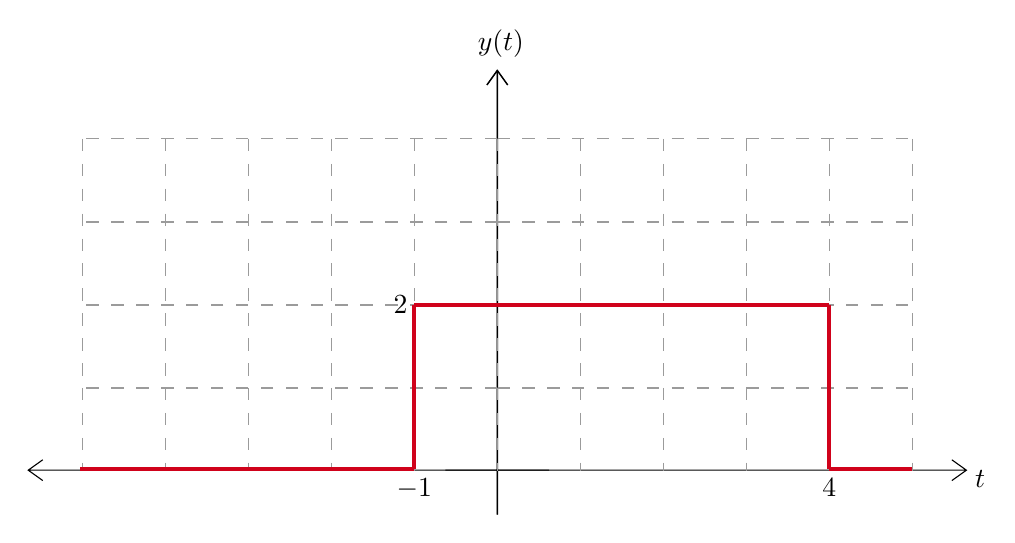
\begin{tikzpicture}[x=0.75pt,y=0.75pt,yscale=-1,xscale=1]
%uncomment if require: \path (0,437); %set diagram left start at 0, and has height of 437

%Shape: Axis 2D [id:dp9049348521282261] 
\draw  (282,282.6) -- (533,282.6)(307.1,90) -- (307.1,304) (526,277.6) -- (533,282.6) -- (526,287.6) (302.1,97) -- (307.1,90) -- (312.1,97)  ;
%Shape: Grid [id:dp1199375004666744] 
\draw  [draw opacity=0][dash pattern={on 4.5pt off 4.5pt}] (307,123) -- (508,123) -- (508,283) -- (307,283) -- cycle ; \draw  [color={rgb, 255:red, 155; green, 155; blue, 155 }  ,draw opacity=1 ][dash pattern={on 4.5pt off 4.5pt}] (307,123) -- (307,283)(347,123) -- (347,283)(387,123) -- (387,283)(427,123) -- (427,283)(467,123) -- (467,283)(507,123) -- (507,283) ; \draw  [color={rgb, 255:red, 155; green, 155; blue, 155 }  ,draw opacity=1 ][dash pattern={on 4.5pt off 4.5pt}] (307,123) -- (508,123)(307,163) -- (508,163)(307,203) -- (508,203)(307,243) -- (508,243) ; \draw  [color={rgb, 255:red, 155; green, 155; blue, 155 }  ,draw opacity=1 ][dash pattern={on 4.5pt off 4.5pt}]  ;
%Shape: Axis 2D [id:dp326465186154436] 
\draw  (332,282.6) -- (81,282.6)(306.9,90) -- (306.9,304) (88,277.6) -- (81,282.6) -- (88,287.6) (311.9,97) -- (306.9,90) -- (301.9,97)  ;
%Shape: Grid [id:dp6083632772154115] 
\draw  [draw opacity=0][dash pattern={on 4.5pt off 4.5pt}] (307,123) -- (106,123) -- (106,283) -- (307,283) -- cycle ; \draw  [color={rgb, 255:red, 155; green, 155; blue, 155 }  ,draw opacity=1 ][dash pattern={on 4.5pt off 4.5pt}] (307,123) -- (307,283)(267,123) -- (267,283)(227,123) -- (227,283)(187,123) -- (187,283)(147,123) -- (147,283)(107,123) -- (107,283) ; \draw  [color={rgb, 255:red, 155; green, 155; blue, 155 }  ,draw opacity=1 ][dash pattern={on 4.5pt off 4.5pt}] (307,123) -- (106,123)(307,163) -- (106,163)(307,203) -- (106,203)(307,243) -- (106,243) ; \draw  [color={rgb, 255:red, 155; green, 155; blue, 155 }  ,draw opacity=1 ][dash pattern={on 4.5pt off 4.5pt}]  ;
%Straight Lines [id:da7648591696995094] 
\draw [color={rgb, 255:red, 208; green, 2; blue, 27 }  ,draw opacity=1 ][line width=1.5]    (467,203) -- (267,203) ;
%Straight Lines [id:da22579692558272613] 
\draw [color={rgb, 255:red, 208; green, 2; blue, 27 }  ,draw opacity=1 ][line width=1.5]    (467,282) -- (467,203) ;
%Straight Lines [id:da14875437832951555] 
\draw [color={rgb, 255:red, 208; green, 2; blue, 27 }  ,draw opacity=1 ][line width=1.5]    (267,282) -- (267,203) ;
%Straight Lines [id:da6615216956994369] 
\draw [color={rgb, 255:red, 208; green, 2; blue, 27 }  ,draw opacity=1 ][line width=1.5]    (267,282) -- (106,282) ;
%Straight Lines [id:da537389837568479] 
\draw [color={rgb, 255:red, 208; green, 2; blue, 27 }  ,draw opacity=1 ][line width=1.5]    (507,282) -- (467,282) ;

% Text Node
\draw (308.72,85) node [anchor=south] [inner sep=0.75pt]    {$y( t)$};
% Text Node
\draw (536,281.4) node [anchor=north west][inner sep=0.75pt]    {$t$};
% Text Node
\draw (267,285.4) node [anchor=north] [inner sep=0.75pt]    {$-1$};
% Text Node
\draw (467,285.4) node [anchor=north] [inner sep=0.75pt]    {$4$};
% Text Node
\draw (265,203) node [anchor=east] [inner sep=0.75pt]    {$2$};


\end{tikzpicture}

        \caption{$y(t)$ Graph}
        \label{fig:5}
      \end{figure}

      The energy over the entire interval may be seen as the function squared, which would be the area under the figure shown above with the height squared (in this case, doubled). This would give us:

      $$\boxed{E_{\infty}=4(5)=20}$$

  \item

    Given the graph of $x(t)$, we know that the slope jumps to $1$ at $t=0$, then $-2$ at $t=1$, then up $2$ at $t=3$, the down $2$ at $t=4$, and so on. This means that we may write this as:

    $$\frac{dx(t)}{dt}=\delta(t)-2\delta(t-1)+2\delta(t-3)-2\delta(t-4)+2\delta(t-6)-2\delta(t-7)+2\delta(t-9)-2\delta(t-10)\cdots$$

    We may group similar terms to write:

    $$\frac{dx(t)}{dt}=\delta(t)-2[\delta(t-1)+\delta(t-4)+\delta(t-7)+\cdots]+2[\delta(t-3)+\delta(t-6)+\delta(t-9)+\cdots]$$

     Noticing a trend, we can write:

    $$\frac{dx(t)}{dt}=\delta(t)-2[\delta(t-1)+\delta(t-1-3k)\cdots]+2[\delta(t-3)+\delta(t-3-3k)\cdots]$$

    Writing this as a summation, we get:

    $$\frac{dx(t)}{dt}=\delta(t)-2\sum_{k=0}^{\infty}\delta(t-1-3k)+2\sum_{k=0}^{\infty}\delta(t-3-3k)$$

    This gives us the coefficients as:

    $$\boxed{A_o=1,\quad A_1=-2,\quad t_1=1,\quad A_2=2,\quad t_2=3}$$

  \item

    The function $x(t)$ may be expressed as:

    $$\boxed{2u(t)-u(t-1)+.5r(t-2)+u(t-4)-.5r(t-4)-2r(t-5)+2r(t-6)-u(t-7)}$$

    Differentiating, we find that $\dfrac{dx(t)}{dt}$ is:

    $$\boxed{2\delta(t)-\delta(t-1)+.5u(t-2)+\delta(t-4)-.5u(t-4)-2u(t-5)+2u(t-6)-\delta(t-7)}$$

    This gives us the following plot:

    \begin{figure}[H]
      \centering
      \tikzset{every picture/.style={line width=0.75pt}} %set default line width to 0.75pt        

\begin{tikzpicture}[x=0.75pt,y=0.75pt,yscale=-1,xscale=1]
%uncomment if require: \path (0,757); %set diagram left start at 0, and has height of 757

%Shape: Grid [id:dp309180394936597] 
\draw  [draw opacity=0][dash pattern={on 4.5pt off 4.5pt}] (181,451) -- (502,451) -- (502,291) -- (181,291) -- cycle ; \draw  [color={rgb, 255:red, 155; green, 155; blue, 155 }  ,draw opacity=1 ][dash pattern={on 4.5pt off 4.5pt}] (181,451) -- (181,291)(221,451) -- (221,291)(261,451) -- (261,291)(301,451) -- (301,291)(341,451) -- (341,291)(381,451) -- (381,291)(421,451) -- (421,291)(461,451) -- (461,291)(501,451) -- (501,291) ; \draw  [color={rgb, 255:red, 155; green, 155; blue, 155 }  ,draw opacity=1 ][dash pattern={on 4.5pt off 4.5pt}] (181,451) -- (502,451)(181,411) -- (502,411)(181,371) -- (502,371)(181,331) -- (502,331) ; \draw  [color={rgb, 255:red, 155; green, 155; blue, 155 }  ,draw opacity=1 ][dash pattern={on 4.5pt off 4.5pt}]  ;
%Shape: Grid [id:dp1199375004666744] 
\draw  [draw opacity=0][dash pattern={on 4.5pt off 4.5pt}] (181,132) -- (502,132) -- (502,292) -- (181,292) -- cycle ; \draw  [color={rgb, 255:red, 155; green, 155; blue, 155 }  ,draw opacity=1 ][dash pattern={on 4.5pt off 4.5pt}] (181,132) -- (181,292)(221,132) -- (221,292)(261,132) -- (261,292)(301,132) -- (301,292)(341,132) -- (341,292)(381,132) -- (381,292)(421,132) -- (421,292)(461,132) -- (461,292)(501,132) -- (501,292) ; \draw  [color={rgb, 255:red, 155; green, 155; blue, 155 }  ,draw opacity=1 ][dash pattern={on 4.5pt off 4.5pt}] (181,132) -- (502,132)(181,172) -- (502,172)(181,212) -- (502,212)(181,252) -- (502,252) ; \draw  [color={rgb, 255:red, 155; green, 155; blue, 155 }  ,draw opacity=1 ][dash pattern={on 4.5pt off 4.5pt}]  ;
%Shape: Axis 2D [id:dp9049348521282261] 
\draw  (144,291.6) -- (517,291.6)(181.3,99) -- (181.3,313) (510,286.6) -- (517,291.6) -- (510,296.6) (176.3,106) -- (181.3,99) -- (186.3,106)  ;
%Shape: Axis 2D [id:dp3810174740882728] 
\draw  (144,291.4) -- (517,291.4)(181.3,484) -- (181.3,270) (510,296.4) -- (517,291.4) -- (510,286.4) (176.3,477) -- (181.3,484) -- (186.3,477)  ;
%Straight Lines [id:da23465514220892947] 
\draw [color={rgb, 255:red, 208; green, 2; blue, 27 }  ,draw opacity=1 ][line width=1.5]    (181.3,291.6) -- (181.01,215) ;
\draw [shift={(181,212)}, rotate = 89.78] [color={rgb, 255:red, 208; green, 2; blue, 27 }  ,draw opacity=1 ][line width=1.5]    (14.21,-4.28) .. controls (9.04,-1.82) and (4.3,-0.39) .. (0,0) .. controls (4.3,0.39) and (9.04,1.82) .. (14.21,4.28)   ;
%Straight Lines [id:da9635494729893386] 
\draw [color={rgb, 255:red, 208; green, 2; blue, 27 }  ,draw opacity=1 ][line width=1.5]    (221.15,291.8) -- (221.01,328) ;
\draw [shift={(221,331)}, rotate = 270.22] [color={rgb, 255:red, 208; green, 2; blue, 27 }  ,draw opacity=1 ][line width=1.5]    (14.21,-4.28) .. controls (9.04,-1.82) and (4.3,-0.39) .. (0,0) .. controls (4.3,0.39) and (9.04,1.82) .. (14.21,4.28)   ;
%Straight Lines [id:da8624510645837334] 
\draw [color={rgb, 255:red, 208; green, 2; blue, 27 }  ,draw opacity=1 ][line width=1.5]    (341.15,271.8) -- (261.15,271.8) ;
%Straight Lines [id:da08847746311409221] 
\draw [color={rgb, 255:red, 208; green, 2; blue, 27 }  ,draw opacity=1 ][line width=1.5]    (341.3,291.6) -- (341.02,255) ;
\draw [shift={(341,252)}, rotate = 89.57] [color={rgb, 255:red, 208; green, 2; blue, 27 }  ,draw opacity=1 ][line width=1.5]    (14.21,-4.28) .. controls (9.04,-1.82) and (4.3,-0.39) .. (0,0) .. controls (4.3,0.39) and (9.04,1.82) .. (14.21,4.28)   ;
%Straight Lines [id:da17568992650795978] 
\draw [color={rgb, 255:red, 208; green, 2; blue, 27 }  ,draw opacity=1 ][line width=1.5]    (421,371) -- (381,371) ;
%Straight Lines [id:da7395813657008669] 
\draw [color={rgb, 255:red, 208; green, 2; blue, 27 }  ,draw opacity=1 ][line width=1.5]    (461.15,291.8) -- (461.01,328) ;
\draw [shift={(461,331)}, rotate = 270.22] [color={rgb, 255:red, 208; green, 2; blue, 27 }  ,draw opacity=1 ][line width=1.5]    (14.21,-4.28) .. controls (9.04,-1.82) and (4.3,-0.39) .. (0,0) .. controls (4.3,0.39) and (9.04,1.82) .. (14.21,4.28)   ;

% Text Node
\draw (182.72,94) node [anchor=south] [inner sep=0.75pt]    {$\frac{dx( t)}{dt}$};
% Text Node
\draw (519,293.4) node [anchor=north west][inner sep=0.75pt]    {$t$};
% Text Node
\draw (341,294.4) node [anchor=north] [inner sep=0.75pt]    {$4$};
% Text Node
\draw (421,294.4) node [anchor=north] [inner sep=0.75pt]    {$6$};
% Text Node
\draw (261,293.4) node [anchor=north] [inner sep=0.75pt]    {$2$};
% Text Node
\draw (501,294.4) node [anchor=north] [inner sep=0.75pt]    {$8$};
% Text Node
\draw (179,212) node [anchor=east] [inner sep=0.75pt]    {$2$};
% Text Node
\draw (179,132) node [anchor=east] [inner sep=0.75pt]    {$4$};
% Text Node
\draw (179,371) node [anchor=east] [inner sep=0.75pt]    {$-2$};
% Text Node
\draw (179,451) node [anchor=east] [inner sep=0.75pt]    {$-4$};


\end{tikzpicture}

      \caption{Plot of $dx(t)/dt$}
      \label{fig:6}
    \end{figure}

  \item

    We can prove linearity by confirming that the input:

    $$x(t)=a_1x_1(t)+a_2x_2(t)$$

    yields output:

    $$y(t)=a_1y_1(t)+a_2y_2(t)$$

    Furthermore, we can prove time invariance by using input:

    $$x(t-t_1)$$

    and confirming this yields output:

    $$y(t-t_1)$$

    \begin{enumerate}[label=\textbf{\alph*)}]

      \item 

        We first define the transformation:

        $$y(t)=2\cos(t)e^{-2t}x(t-2)$$

        For linearity, $x(t-2)=a_1x_1(t)+a_2x_2(t)$ should yield:

        $$2a_1\cos(t)e^{-2t}x_1(t-2)+2a_2\cos(t)e^{-2t}x_2(t-2)$$

        Checking $a_1y_1(t)+a_2y_2(t)$, we see:

        $$a_1y_1(t)+a_2y_2(t)=2a_1\cos(t)e^{-2t}x_1(t-2)+2a_2\cos(t)e^{-2t}x_2(t-2)$$

        Since the two are equivalent, \underline{the transform is linear}. We now check for time invariance:

        $$x(t-t_1)\to2\cos(t)e^{-2t}x(t-2-t_1)$$
        $$y(t-t_1)\to2\cos(t-t_1)e^{-2(t-t_1)}x(t-2-t_1)$$

        Since $x(t-t_1)\neq y(t-t_1)$, \underline{the transform is not time invariant}

      \item 

        We first define the transform:

        $$y[n]=x[n-4]+2n^2x[n-2]$$

        Checking for linearity, we test $a_1x_1[n]+a_2x_2[n]$:

        $$a_1x_1[n-4]+2a_1n^2x_1[n-2]+a_2x_2[n-4]+2a_2n^2x_2[n-2]$$

        Comparing to $a_1y_1[n]+a_2y_2[n]$, we see:

        $$a_1x_1[n-4]+2a_1n^2x_1[n-2]+a_2x_2[n-4]+2a_2n^2x_2[n-2]$$

        Since the two are the same, \underline{the transform is linear}. We now check for time invariance:

        $$x[n-n_o]\to x[n-4-n_o]+2n^2x[n-2-n_o]$$
        $$y[n-n_o]\to x[n-4-n_o]+2(n-n_o)^2x[n-2-n_o]$$

        Since $x[n-n_o]\neq y[n-n_o]$, \underline{the transform is not time invariant}

      \item 

        First, we define the transform:

        $$y[n]=2x^2[n-1]$$

        Checking for linearity, we test $a_1x_1[n]+a_2x_2[n]$:

        $$2a_1^2x_1^n[n-1]+2a_2^2x_2^2[n-1]+4a_1a_2x_1[n-1]x_2[n-1]$$

        Comparing to $a_1y_1[n]+a_2y_2[n]$, we see:

        $$2a_1x_1^n[n-1]+2a_2x_2^2[n-1]$$

        Since the two are not equivalent, \underline{the transform is not linear}. Now we check for time invariance:

        $$x[n-n_o]\to 2x^2[n-1-n_o]$$
        $$y[n-n_o]\to 2x^2[n-1-n_o]$$

        Since the two are equivalent, \underline{the transform is time invariant}

    \end{enumerate}

  \item

    \begin{enumerate}[label=\textbf{\alph*.}]

      \item 

        By inspection, we can see that the transform can be written as:

        $$y(t)=2x\left( t-\frac{\pi}{12} \right)$$

        Testing this system, we see:

        $$2e^{j\left[ 3\left( t-\dfrac{\pi}{12} \right) \right]}=2e^{-\frac{j\pi}{4}}e^{3jt}$$
        $$2e^{j\left[ -3\left( t-\dfrac{\pi}{12} \right) \right]}=2e^{\frac{j\pi}{4}}e^{-3jt}$$

        Taking $x_1(t)=4\cos(3t)$ as the input, we find that the output is:

        $$\boxed{y_1(t)=8\cos\left( 3t-\frac{\pi}{4} \right)}$$

      \item 

        Taking $x_2(t)=2\sin\left(3t-\frac{\pi}{2}\right)$ as the input, we find that the output is:

        $$\boxed{y_2(t)=4\sin\left( 3t-\frac{3\pi}{4} \right)}$$

    \end{enumerate}

  \item

    \begin{enumerate}[label=\textbf{\alph*)}]

      \item 

        For $x_1(t)=\pi/4$ and $x_2(t)=(9\pi/4)$, $y(t)$ has the same output:

        $$y_1(t)=2\cos\left( \frac{\pi}{4}-\frac{\pi}{4} \right)=2$$
        $$y_2(t)=2\cos\left( \frac{9\pi}{4}-\frac{\pi}{4} \right)=2$$

        Therefore, \underline{the transform is not invertible}

      \item 

        \underline{This system is invertible}. We may write:

        $$x[n]=\left\{\begin{matrix} x[n], & n > 1\\ x[n+1], & n \leq 1\end{matrix}$$

      \item 

        We can begin to manipulate the system as:

        $$y\left( \frac{t}{4} \right)=e^{.5t}x(t)$$
        $$x(t)=e^{-.5t}y\left( \frac{t}{4} \right)$$

        Thus, we see that \underline{the system is invertible}

    \end{enumerate}

  \item

    \begin{enumerate}

      \item 

        For $x_2(t)$, we see that the input is shifted 1 unit to the left, and doubled in magnitude. Additionally, we add a part that is shifted 1 unit right, with an opposite magnitude. Thus, we write:

        $$x_2(t)=2x_1(t+1)-x_1(t-1)$$

        According to linearity and time invariance, we know the output will respond as:

        $$\boxed{y_2(t)=2y_1(t+1)-y_1(t-1)}$$

        This gives us the following graph:

        \begin{figure}[H]
          \centering
          \tikzset{every picture/.style={line width=0.75pt}} %set default line width to 0.75pt        

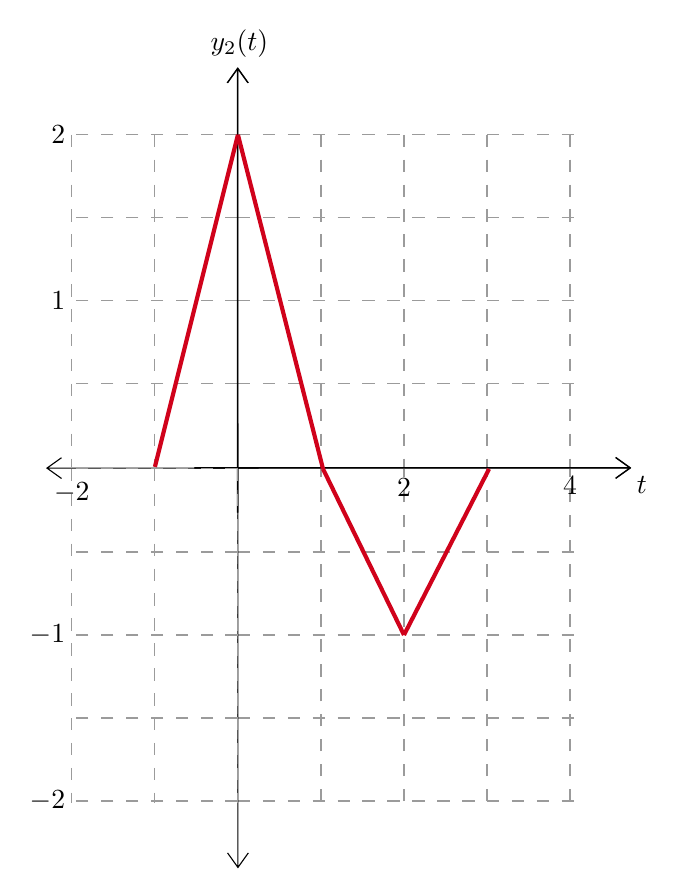
\begin{tikzpicture}[x=0.75pt,y=0.75pt,yscale=-1,xscale=1]
%uncomment if require: \path (0,757); %set diagram left start at 0, and has height of 757

%Shape: Grid [id:dp1199375004666744] 
\draw  [draw opacity=0][dash pattern={on 4.5pt off 4.5pt}] (235,131) -- (397,131) -- (397,291) -- (235,291) -- cycle ; \draw  [color={rgb, 255:red, 155; green, 155; blue, 155 }  ,draw opacity=1 ][dash pattern={on 4.5pt off 4.5pt}] (235,131) -- (235,291)(275,131) -- (275,291)(315,131) -- (315,291)(355,131) -- (355,291)(395,131) -- (395,291) ; \draw  [color={rgb, 255:red, 155; green, 155; blue, 155 }  ,draw opacity=1 ][dash pattern={on 4.5pt off 4.5pt}] (235,131) -- (397,131)(235,171) -- (397,171)(235,211) -- (397,211)(235,251) -- (397,251) ; \draw  [color={rgb, 255:red, 155; green, 155; blue, 155 }  ,draw opacity=1 ][dash pattern={on 4.5pt off 4.5pt}]  ;
%Shape: Axis 2D [id:dp9049348521282261] 
\draw  (214,291.6) -- (424,291.6)(235,99) -- (235,313) (417,286.6) -- (424,291.6) -- (417,296.6) (230,106) -- (235,99) -- (240,106)  ;
%Shape: Grid [id:dp38260027148349784] 
\draw  [draw opacity=0][dash pattern={on 4.5pt off 4.5pt}] (235,131) -- (153,131) -- (153,291) -- (235,291) -- cycle ; \draw  [color={rgb, 255:red, 155; green, 155; blue, 155 }  ,draw opacity=1 ][dash pattern={on 4.5pt off 4.5pt}] (235,131) -- (235,291)(195,131) -- (195,291)(155,131) -- (155,291) ; \draw  [color={rgb, 255:red, 155; green, 155; blue, 155 }  ,draw opacity=1 ][dash pattern={on 4.5pt off 4.5pt}] (235,131) -- (153,131)(235,171) -- (153,171)(235,211) -- (153,211)(235,251) -- (153,251) ; \draw  [color={rgb, 255:red, 155; green, 155; blue, 155 }  ,draw opacity=1 ][dash pattern={on 4.5pt off 4.5pt}]  ;
%Shape: Axis 2D [id:dp509145843401392] 
\draw  (245,291.6) -- (143,291.6)(234.8,99) -- (234.8,313) (150,286.6) -- (143,291.6) -- (150,296.6) (239.8,106) -- (234.8,99) -- (229.8,106)  ;
%Shape: Grid [id:dp3116070310441251] 
\draw  [draw opacity=0][dash pattern={on 4.5pt off 4.5pt}] (235,452) -- (397,452) -- (397,292) -- (235,292) -- cycle ; \draw  [color={rgb, 255:red, 155; green, 155; blue, 155 }  ,draw opacity=1 ][dash pattern={on 4.5pt off 4.5pt}] (235,452) -- (235,292)(275,452) -- (275,292)(315,452) -- (315,292)(355,452) -- (355,292)(395,452) -- (395,292) ; \draw  [color={rgb, 255:red, 155; green, 155; blue, 155 }  ,draw opacity=1 ][dash pattern={on 4.5pt off 4.5pt}] (235,452) -- (397,452)(235,412) -- (397,412)(235,372) -- (397,372)(235,332) -- (397,332) ; \draw  [color={rgb, 255:red, 155; green, 155; blue, 155 }  ,draw opacity=1 ][dash pattern={on 4.5pt off 4.5pt}]  ;
%Shape: Axis 2D [id:dp9445758822579701] 
\draw  (214,291.4) -- (424,291.4)(235,484) -- (235,270) (417,296.4) -- (424,291.4) -- (417,286.4) (230,477) -- (235,484) -- (240,477)  ;
%Straight Lines [id:da09039927216219223] 
\draw [color={rgb, 255:red, 208; green, 2; blue, 27 }  ,draw opacity=1 ][line width=1.5]    (195,291) -- (235,131) ;
%Straight Lines [id:da9718155597929978] 
\draw [color={rgb, 255:red, 208; green, 2; blue, 27 }  ,draw opacity=1 ][line width=1.5]    (235,131) -- (276,292) ;
%Straight Lines [id:da4117833381221786] 
\draw [color={rgb, 255:red, 208; green, 2; blue, 27 }  ,draw opacity=1 ][line width=1.5]    (276,292) -- (315,372) ;
%Shape: Grid [id:dp7431999536611184] 
\draw  [draw opacity=0][dash pattern={on 4.5pt off 4.5pt}] (235,292) -- (153,292) -- (153,453) -- (235,453) -- cycle ; \draw  [color={rgb, 255:red, 155; green, 155; blue, 155 }  ,draw opacity=1 ][dash pattern={on 4.5pt off 4.5pt}] (235,292) -- (235,453)(195,292) -- (195,453)(155,292) -- (155,453) ; \draw  [color={rgb, 255:red, 155; green, 155; blue, 155 }  ,draw opacity=1 ][dash pattern={on 4.5pt off 4.5pt}] (235,292) -- (153,292)(235,332) -- (153,332)(235,372) -- (153,372)(235,412) -- (153,412)(235,452) -- (153,452) ; \draw  [color={rgb, 255:red, 155; green, 155; blue, 155 }  ,draw opacity=1 ][dash pattern={on 4.5pt off 4.5pt}]  ;
%Straight Lines [id:da43129718422211005] 
\draw [color={rgb, 255:red, 208; green, 2; blue, 27 }  ,draw opacity=1 ][line width=1.5]    (356,292) -- (315,372) ;

% Text Node
\draw (235.72,95) node [anchor=south] [inner sep=0.75pt]    {$y_{2}( t)$};
% Text Node
\draw (426,294.4) node [anchor=north west][inner sep=0.75pt]    {$t$};
% Text Node
\draw (395,294.4) node [anchor=north] [inner sep=0.75pt]    {$4$};
% Text Node
\draw (315,295.4) node [anchor=north] [inner sep=0.75pt]    {$2$};
% Text Node
\draw (153,211) node [anchor=east] [inner sep=0.75pt]    {$1$};
% Text Node
\draw (153,131) node [anchor=east] [inner sep=0.75pt]    {$2$};
% Text Node
\draw (155,297.4) node [anchor=north] [inner sep=0.75pt]    {$-2$};
% Text Node
\draw (153,372) node [anchor=east] [inner sep=0.75pt]    {$-1$};
% Text Node
\draw (153,452) node [anchor=east] [inner sep=0.75pt]    {$-2$};


\end{tikzpicture}

          \caption{Output $y_2(t)$ for Input $x_2(t)$}
          \label{fig:7}
        \end{figure}

      \item 

        For $x_3(t)$, we see that the transform is:

        $$x_3(t)=2x_1\left( 2t \right)-2x_1(2t-4)$$

        This gives us output:

        $$\boxed{y_3(t)=2y_1\left( 2t \right)-2y_1(2t-4)}$$

        Which produces the following graph:

        \begin{figure}[H]
          \centering
          \include{Figures/H2P9b}
          \caption{Output $y_3(t)$ for Input $x_3(t)$}
          \label{fig:8}
        \end{figure}

    \end{enumerate}

\end{enumerate}

\end{document}

